Large language models suffer from several fundamental issues, which are not entirely solvable through training or prompt engineering. 
\citet{Gao.18.12.2023} stated that LLMs have significant limitations in knowledge-intesive or domain-specific tasks. Missing or unsufficient amount of information on a specific subject while training lead to wrong answers. For large language models this is called \textit{hallucinations} as defined in \citet{Huang.2023}. For retrieval-augmented generation systems (RAGs) the term hallucinations is defined for stating information without context. \citet{Rashkin.} defined hallucinations as any information that is neither inferable from nor stated by an external document. In this thesis I will use the definition for RAG systems. 

Factual wrong output from an LLM can have several reasons. The required information to answer this question can be private, stored on a database that is not accessible during training. Another reason might be that training or fine-tuning the model is expensive and thus done less frequent. Therefore the required information can be published more recently then the last training run. All those problems can be solved if the LLM is not used for the answer itself, but rather used for building a coherent text passage given a question and its answer. Then a database would store all relevant information and would be updated as frequent as required. At inference time the prompt is used to determine relevant chunks of documents within the database, which are then used for the generation of the answer.

This concept is very successful as \citet{Shuster.} showed. Factual wrong outputs are reduced and open-domain conversational capabilities are increased. \citet{Yu.2024} concluded that this improves the reliability and richnes of the produced content. \citet{Chen.2024} stated that external knowledge would be the key for resolving the above stated problems of LLMs, which make them more accurate and reliable.

There is a high variety in architectures and approaches for retrieval-augmented generation models. In this section, I will give an overview of the most common approaches and architectures and start with the most basic ones. The section will follow the definition of RAGs in \citet{Gao.18.12.2023} with naive RAGs, advanced RAGs, a modular architecture, and special cases. 

\subsection{Naive RAGs}
\label{sec:naive_rags}
Naive RAGs can be seen as the most basic form of a retrieval-augmented generation system. The core idea behind this concept is to give all relevant context for answering a question or solving a task into the prompt for the large language model. Then the LLM is only used for generating a coherent answer. Therefore it is required to ingest relevant data for the given use case beforehand. The system then retrieves relevant chunks or documents of this data at inference time. 


\begin{figure}[h!]
    \centering
    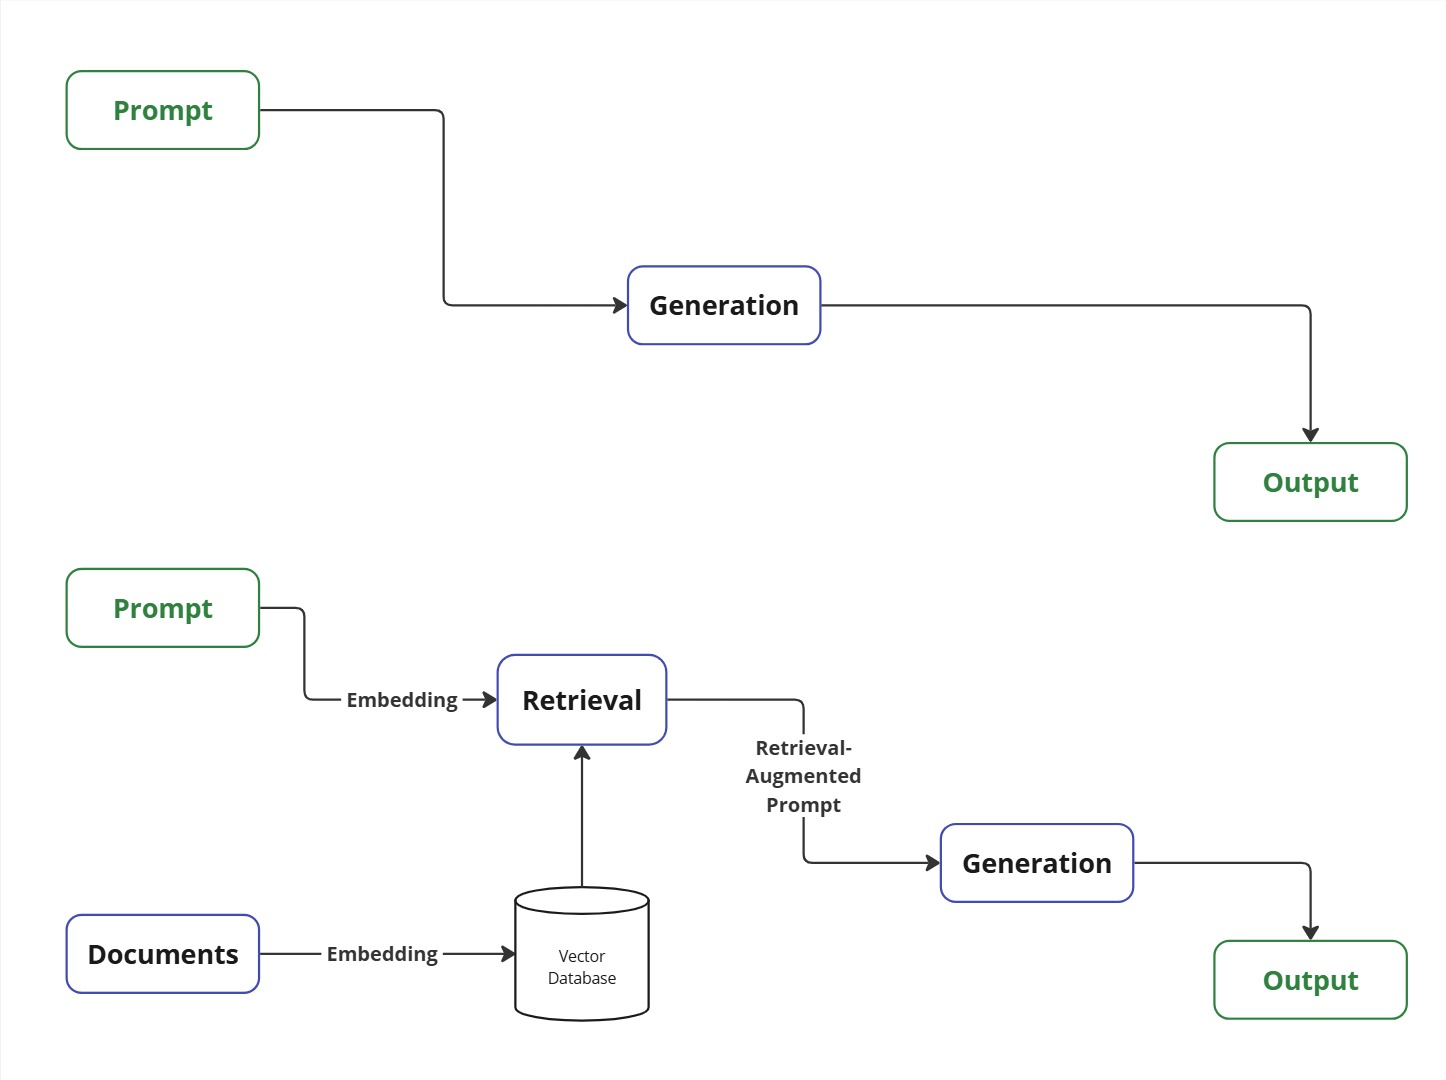
\includegraphics[width=\textwidth]{images/LLM-vs-RAG.jpg}
    \caption{Comparison of the process to the prompt, above a standalone LLM that has a prompt and generate a response, below a RAG system that performs on a given set of documents an embedding or indexing and searchs for the most similar documents for a given prompt at inference time. Both prompt and documents are used for the generation process.}
    \label{fig:naive_rag}
\end{figure}

This procedure can be seen in figure \ref{fig:naive_rag}. In the literature the generation process is often refered as \textit{read}, because it reads the prompt and the provided context. In \citet{Gao.18.12.2023} they define the naive RAG system as \textit{Retrieve-Read}. The retrieval can be done with sparse retrieval (TF-IDF, BM25), dense retrieval (DPR) or a hybrid version as showed in section \ref{retrieval}. 

\begin{figure}[h!]
    \centering
    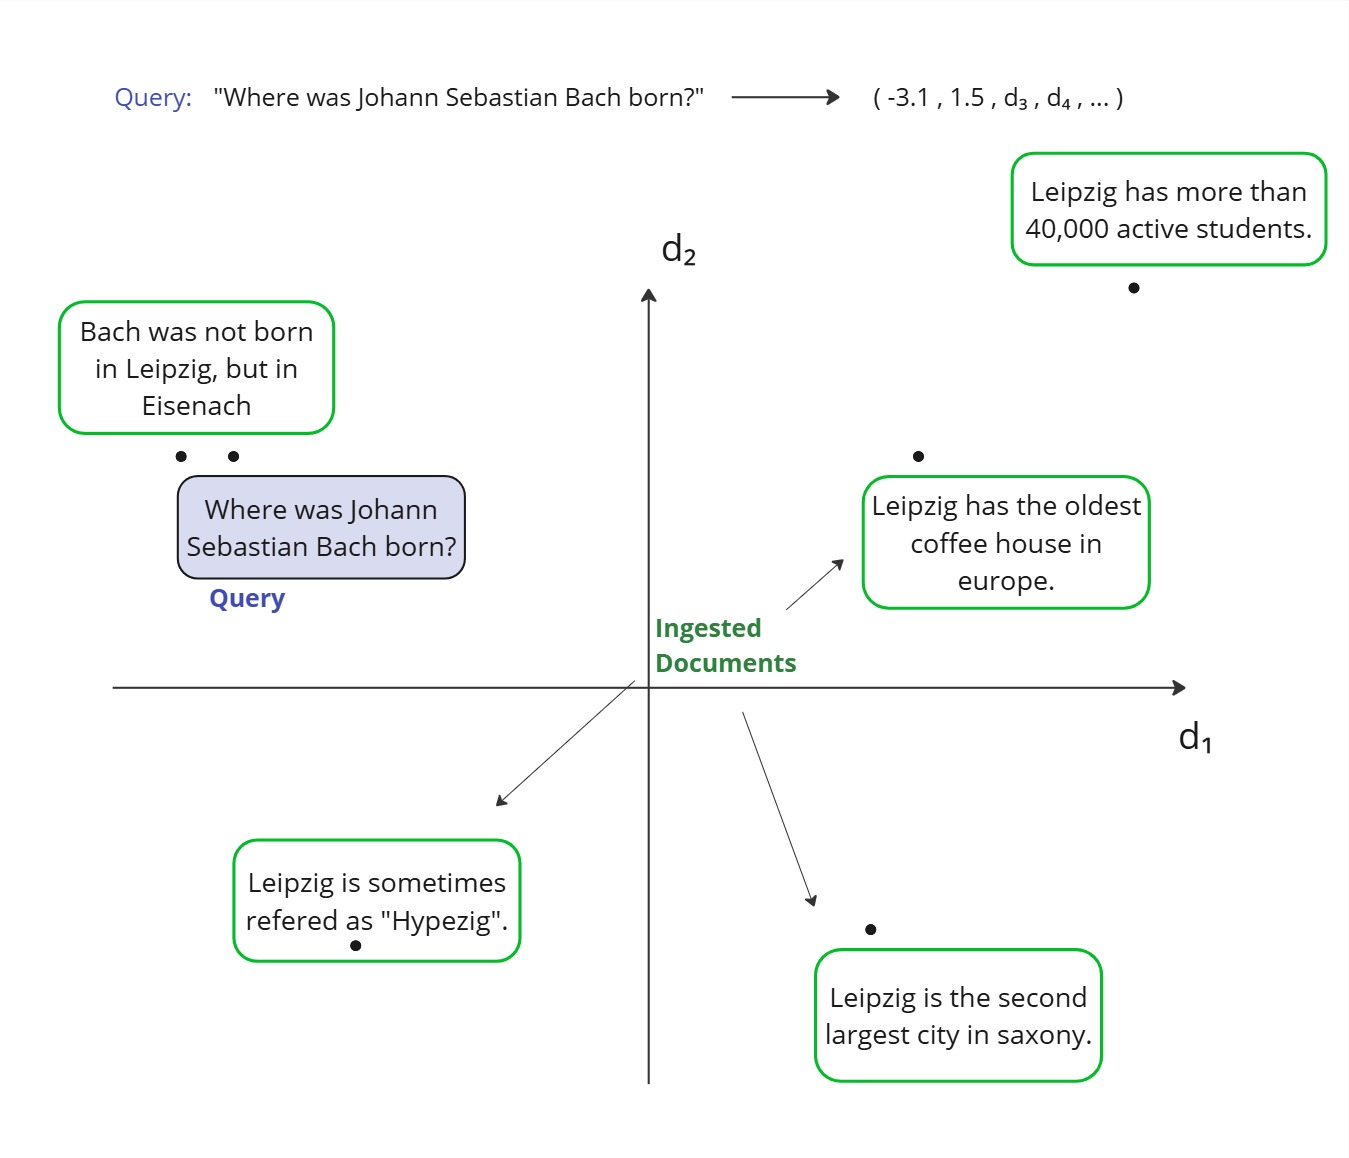
\includegraphics[width=\textwidth]{images/VectorDB.jpg}
    \caption{A vector space including mapped facts (documents) and a user query. The query and its correct answer have similar vectors}
    \label{fig:vectorDB}
\end{figure}


Before the system can be used, it is necessary to ingest data. The ingestion process includes preprocessing and selection of data, that users are likely to need for their questions or use-cases. Therefore it is relevant to know the user base. It is not feasible nor efficient to ingest all availlable data. The data is transformed into documents or chunks of documents. There are multiple ways to do this, which are described in advanced techniques. As described in \ref{sec:dense_retrieval}, the chunks are then encoded and mapped into a d-dimensional real-valued vector space. There is a simplistic minimal example of a vector space in figure \ref{fig:vectorDB}. The documents gets mapped in different loactions within the space. The assumption is, that the embedding model will map correct answers to the corresponding queries. In reality there will be more documents close to each other, documents and queries are longer or more complex and each query will return the "Top-K" chunks or documents, which are not always as relevant as in this example. Top-K can be seen as hyperparamter for the system. 

The vectors are then stored in so called vector databases. Such databases are specialized and include functionalities like inverted indices, clustering of precomputed vector similarities, approximate nearest neighbor algorithm, hierarchical navigable small world and quantizations, which will not be covered in this master thesis.  


\citet{Gao.18.12.2023} listed several drawbacks for naive RAGs. The basic retrieval suffers from unsufficient recall and precision scores leading in irrelevant documents, missing context and bias. The integration of the provided context is a challenging process. The generator often overrelies on the augmented information, by just repeating the retrieved content and missing insightful conclusions. Therefore this simplistic form of RAG needs advanced techniques to overcome those issues. 

\subsection{Advanced RAGs}
\label{sec:advanced_rags}

There is no strict definition of advanced versions of retrieval-augmented generation systems. The term describes a loose bundle of techniques to improve the quality of such systems. Following is a list, which items I will explain in greater details afterwards.

\paragraph{Chunking}
\label{sec:chunk}
% graphic for techniques, such as overlap, fixed sized (sliding window approach), semantic chunks, ...
For understanding the necessarity of chunking it is helpful to illustrate it with a following example. Let us use a sentence from \citeauthor{LeipzigWikipedia.2025} for Leipzig from \citeyear{LeipzigWikipedia.2025}. In the section "Music" there is the following sentence. 

\begin{quote}
    "Johann Sebastian Bach spent the longest phase of his career in Leipzig, from 1723 until his death in 1750, conducting the Thomanerchor (St. Thomas Church Choir), at the St. Thomas Church, the St. Nicholas Church and the Paulinerkirche, the university church of Leipzig (destroyed in 1968)."
\end{quote}

If there are thousands of wikipedia pages or websites to process, then this can not be splitted manually. What is the document or a good chunk in this context. If the query asks if Johann Sebastian Bach lived in Leipzig, then embedding the whole sentence would not guarantee a high similarity vector score in the retrieval process. This differs from domain to domain. While chunking facts from sentences might be a valid strategy for wikipedia, processing internal contracts in a large company would need less granular chunking. 

Therefore there are several chunking techniques to consider for tuning the RAG-system. Fixed-Size chunking splits a document after a fixed size of characters, e. g. every 400 characters a chunk ends and a new one starts. The sliding window approach adds a overlap of few characters. Semantic Chunking splits with prior defined characters such as "\textit{$\backslash n$, $\backslash\backslash n$ or <br>}". There are also special use-case techniques such as Markdown, JSON, HTML and programming code chunkers. Almost all presented chunking techniques are offered in typical libraries e. g. Llama-Index (\citet{Liu_LlamaIndex_2022}) or Langchain (\citeauthor{Chase_LangChain_2022}).

Additional to advanced chunking, it is recommended to enrich the resulting documents with metadata, which can be used at inference time for filtering. 

% ToDo: 
% - Just Write them Down!
% - Drawbacks
% - Point of Failures in RAGs
% - Überleitung zu Evaluation

\paragraph{Rewrite}
\label{sec:rewrite}
% Query Rewriting, Query Transformation, Query Expansion (see. papers)

\paragraph{Rerank}
\label{sec:rerank}
% Reranking Techniques, Lost-in-The-Middle?, Diversity Ranking, ... 

\paragraph{Iterative RAGs}
\label{sec:iterative}
% Short description with graphic

\paragraph{Recursive RAGs}
\label{sec:recursive}
% Short description with graphic

\paragraph{Adaptive RAGs}
\label{sec:adaptive}
% Short description with graphic

\subsection{General Modular RAG}
\label{sec:modular_rag}
% The core idea behind it, to be as flexible as possible and bridge to special cases

\subsection{Special Cases}
\label{sec:special_cases}
% short list of special cases

\subsection{Drawbacks of RAGs}
\label{sec:drawbacks}
